%**************************************************************************************
\subsection{Simulation Stories - Introduction}
%**************************************************************************************

%**************************************************************************************
\subsubsection{MediTransCare - About the company}
%**************************************************************************************
MediTransCare is a company specialized on medical goods settled in Vienna. Its custom-ers are distributed all over Europe. The emphasis of the enterprise is on secure and in-time delivery of medical goods. For this purpose MediTransCare owns a distribution and storage network across Europe.
\\\\
In the field of "medical logistics" it is vital not to break the cold chain of pharmaceuticals or to overrun the expiry date. During transportation and temporary storage pharmaceuti-cals can be exposed to heavy surrounding conditions that can damage the goods. Fur-thermore the products have to be secured against theft (abuse).
\\\\
The requirement in the medical supply field grows more than ever and the requirements on logistics in reference to an economic distribution forms here the emphasis.  Many cus-tomers appreciate a just-in-time delivery whereby special attention is set on that no bot-tlenecks or over-capacities arise locally.
\\\\
The company makes extensive use of IT systems that can identify and predict future needs and demands of its customers. It can create profiles out of behaviour patterns and seasonal empirical values. Thus it can recognize automatically that a shortage on sup-plies is going to become apparent and deploy counter measures to avoid such situations. It can order buffer deliveries, store and secure them and in case of demand deliver the products within hours to its customers.
\\\\
MediTransCare selects among reliable carriers based on economical aspects to deliver their products.  The carriers have to be able to accomplish the assignment within the specified conditions (e.g. special cooling, delivery date). Together with the carriers MediTransCare works out an exact delivery plan to ensure that the delivery arrives in time.
\\\\
The buffer of pharmaceuticals is secured through a network of local storage depots that can assure the high standards required by storing pharmaceuticals. Local carriers can de-liver the ordered goods within hours to the customers.
\\\\
Basically MediTransCare is able to deliver products in Europe within 4 to 7 days from one depot storage to another one. The means of transport are either by truck or by cargo planes depending on the requirements.
\\\\
The whole delivery process is under constant surveillance to be able to react on problems like quality, delivery delays or loss.

%**********************
\begin{figure}[!h]                               
	\centering                                           
	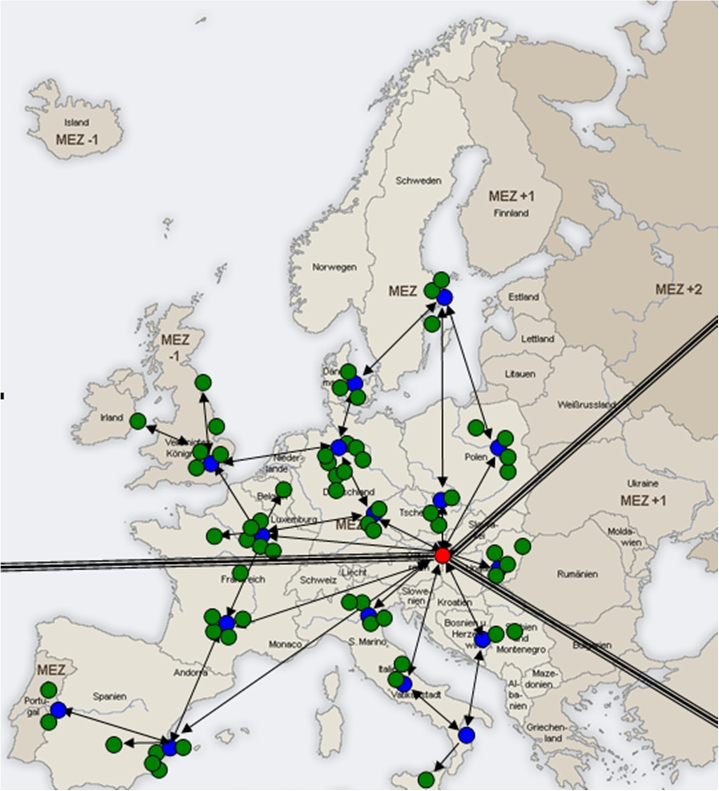
\includegraphics[width=1\textwidth]{pics/europeMap.jpg}
	\caption{MediTransCare's transportation network}             
	\label{fig:MediTransCaretransportationnetwork}
\end{figure}  
%**********************

%**************************************************************************************
\subsubsection{The delivery process}
%**************************************************************************************
The basic phases during a delivery process look like as follows:

\begin{itemize}
	\item Load Planning 
	\item Load Tendering
	\item Carrier Dispatch and Load
	\item InTransit - Track and Trace
\end{itemize}
In the following sections the process of a delivery between local storage depots will be explained. This process starting from an incoming order to the final delivery at the de-sired destination is described in the following sections.

%**************************************************************************************
\subsubsection{The Offer}
%**************************************************************************************
A local storage depot requests a delivery of one or more products if the stock level sinks under a predefined threshold, a higher demand is expected or you get a big order from a customer. Usually this is done through an IT system. The order will be handed over to a proper coordinator (Transportation Planner) who is responsible for planning and dispatch-ing outgoing supplies. He will handle the order further on.

%**************************************************************************************
\subsubsection{Load Tendering}
%**************************************************************************************
The Transportation Planner forwards the offer with its cargo characteristics and the gen-eral conditions to a pool of carriers.
\\\\
For almost all deliveries going out from MediTransCare a cooling is required for the cargo, because almost every medical good has to stay between a temperature-interval in order to ensure the quality.
\\\\
It also can happen that a transport needs two different temperature zones for pharma-ceutics that require a different cooling temperature. This would require special equipment to create two different climate chambers. These requirements have to be announced to all carriers so that they can prepare their equipment or to check their utilization.
\\\\
The contacted carriers have to reply within a specific time period if they want to accept or reject the offer.
%**************************************************************************************
\subsubsection{Load Planning}
%**************************************************************************************
Right after the decision has been made which carrier will perform the delivery, a detailed plan is developed together with the selected carrier that defines exactly how the trans-port will be executed.
\\\\
This plan contains the sections with the stops and reloads on the way to the target desti-nation. For example a cargo from Vienna to Madrid would take the route from Vienna to Munich and then from Munich to Madrid. Over night the cargo has to be stored in the de-pot in Munich.
\\\\
To be able to control and track the transport you need more information besides delivery dates. There is a definition for buffer times for each section on the route. With these times it is possible to identify imminent delays. 

%**************************************************************************************
\subsubsection{Carrier Dispatch and Load}
%**************************************************************************************
The medical supplies are usually packed between polystyrene boxes layered up in boxes. If necessary the cargo is cooled with dry ice during packaging. 

%**********************
\begin{figure}[!h]                               
	\centering                                           
	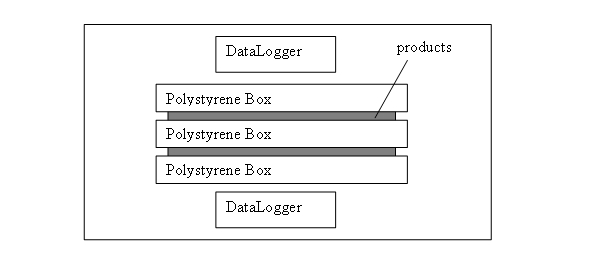
\includegraphics[width=1\textwidth]{pics/transportBox.jpg}
	\caption{Polystyrene package}             
	\label{fig:Polystyrene package}
\end{figure}  
%**********************

Multiple dataloggers are packed between the stacked boxes to measure every 60 minutes (standard value) the temperature to achieve meaningful results. With these measure-ments you can ensure the quality of the products after a transportation.
\\\\
Dataloggers are programmed with following data before they are packed into the cargo:

\begin{itemize}
	\item Logger Id
	\item Order Id
	\item Destination
	\item Min-Max temperature threshold
	\item How often should the datalogger measure the temperature (Standard: every 60min)
	\item Person who has programmed the datalogger
\end{itemize}

A datalogger has a maximal capacity of 200 measurements which means that the trans-port duration is limited if you want to ensure the product's quality.

%**************************************************************************************
\subsubsection{InTransit - Track and Trace}
%**************************************************************************************
The cargo is handed over to the contracted carrier at the beginning. 
\\\\
The transport goes usually over several stages where the supplies have to be reloaded. Like: 
\\\\
The transport goes over several stations by truck or by train to the desired destination.
The carrier reloads the shipment on a cargo plane. Arrived at the flight destination the cargo is reloaded again onto a local carrier truck that brings the shipment to the destina-tion.
\\\\
At the end of each section the delivery is checked. On one hand the correctness of the quantity is controlled and on the other hand the quality of the products. The delivery has to be in the planned delivery time.
\\\\
The quality control is done by examining the dataloggers to ensure that the last stage went alright and the products haven't been exposed to illegal temperatures.

%**************************************************************************************
\subsubsection{Acceptance of Shipment}
%**************************************************************************************
When the product arrived at the destination a storage depot staffmember examines the cargo. The shipment has to be complete and visually alright. Afterwards the dataloggers are taken out for an analysis (e.g. measured temperatures are read out). 
\\\\
If the measurements are valid too and the shipment was delivered in time than the transport is booked as a success and is completed.

%**************************************************************************************
\subsubsection{Process-events}
%**************************************************************************************
In this section the events are described that are generated during a process flow.
\\\\
\textbf{OrderReceived} (OrderId, DateTime, DeliveryDate, Destination, ProductCollection)\\
This event occurs if a new order has been generated.
\begin{mytinylisting}
	\begin{verbatim}
<OrderReceived>
		<OrderId>14765</OrderId>
		<DateTime>2005-10-31T11:31:02</DateTime>
		<DeliveryDate>2005-11-12T06:00:00</DeliveryDate>
		<Destination>Madrid</Destination>
		<ProductCollection>
			<Product>		
    	<ProductId>Arzeutic</ProductId>
	<Amount>700</Amount>
</Product>	
		</ProductCollection>
</OrderReceived>
\end{verbatim}
\end{mytinylisting}


\textbf{OrderConfirmed} (OrderId, DateTime)\\
This event occurs if an offer has been confirmed.
\begin{mytinylisting}
\begin{verbatim}
<OrderConfirmed>
		<OrderId>14765</OrderId>
		<DateTime>2005-10-31T13:45:17</DateTime>
</OrderConfirmed>
\end{verbatim}
\end{mytinylisting}


\textbf{ShipmentTenderIssued} (OrderId, DateTime, FurtherInfo) \\
The order including conditions and constraints is sent to a pool of carriers.
\begin{mytinylisting}
\begin{verbatim}
<ShipmentTenderIssued>
	<OrderId>14765</OrderId>
	<DateTime>2005-10-31T14:12:54</DateTime>
	<FurtherInfo>
		<ShipmentInfo>		
    	<From>Vienna</From>
	<To>Madrid</To>
	<DeliveryDate>2005-11-12T06:00:00</DeliveryDate>
	<TransportType>Truck</TransportType>
	<Price>2500</Price>
	<MinTemp>3</MinTemp>
	<MaxTemp>8</MaxTemp>
</ShipmentInfo>
	</FurtherInfo>
</ShipmentTenderIssued>	
\end{verbatim}
\end{mytinylisting}


\textbf{ShipmentTenderAccepted} (OrderId, CarrierId, DateTime)\\
The carrier accepts the tender.
\begin{mytinylisting}
\begin{verbatim}
<OrderConfirmed>
	<OrderId>14765</OrderId>
	<CarrierId>433</CarrierId>
	<DateTime>2005-10-31T13:45:17</DateTime>
</OrderConfirmed>	

\end{verbatim}
\end{mytinylisting}


\textbf{ShipmentTenderRejected} (OrderId, CarrierId, DateTime)\\
The carrier rejects the tendered transport under the given conditions.
\begin{mytinylisting}
\begin{verbatim}
<ShipmentTenderRejected> 
		<OrderId>14765</OrderId>
		<CarrierId>532</CarrierId>
		<DateTime>2005-10-31T15:12:21</DateTime>
</ShipmentTenderRejected>
\end{verbatim}
\end{mytinylisting}


\textbf{ShipmentCreated} (OrderId, TransportId, CarrierId, DateTime, DatePlannedShipped, DatePlannedDelivered, DateEarlyBuffered, DateLateBuffered, LocationFrom, LocationTo, Miles, PlannedFreightCosts, TransportType)\\
The shipment specifications worked out together with the carrier. These values mark a successful delivery and they are controlled by the system. A shipment can contain more than one stage ("TransportInfo", TransportStart-TransportEnd).
\begin{mytinylisting}
\begin{verbatim}
<ShipmentCreated> 
	<OrderId>14765</OrderId>
	<DateTime>2005-10-31T15:45:25</DateTime>
      <Transport>
<TransportInfo>
      <TransportId>42322</TransportId>
	<CarrierId>433</CarrierId>
	<DatePlannedShipped>2005-11-07T08:15:00</DatePlannedShipped>
	<DatePlannedDelivered>2005-11-7T17:00:00</DatePlannedDelivered>
	<DateEarlyBuffered>2005-11-06T16:00:00</DateEarlyBuffered>
	<DateLateBuffered>2005-11-08T06:00:00</DateLateBuffered>
	<LocationFrom>Vienna</LocationFrom>
	<LocationTo>Munich</LocationTo>
	<Miles>422</Miles>
	<PlannedFreightCosts>690</PlannedFreightCosts>
	<TransportType>Truck</TransportType>
</TransportInfo>
<TransportInfo>
      <TransportId>42323</TransportId>
	<CarrierId>433</CarrierId>
	<DatePlannedShipped>2005-11-08T14:00:00</DatePlannedShipped>
	<DatePlannedDelivered>2005-11-0T17:00:00</DatePlannedDelivered>
	<DateEarlyBuffered>2005-11-07T17:00:00</DateEarlyBuffered>
	<DateLateBuffered>2005-11-12T06:00:00</DateLateBuffered>
	<LocationFrom>Munich</LocationFrom>
	<LocationTo>Madrid</LocationTo>
	<Miles>1810</Miles>
	<PlannedFreightCosts>690</PlannedFreightCosts>
	<TransportType>Truck</TransportType>
</TransportInfo>
      </Transport>
</ShipmentCreated>
\end{verbatim}
\end{mytinylisting}


\textbf{DataLoggerConfigured} (OrderId, LoggerId, DateTime, Staffmember, MinTemp, MaxTemp, SenseInterval, Destination)\\
Datalogger settings for shipment monitoring.
\begin{mytinylisting}
\begin{verbatim}
<DataLoggerConfigured>
	<OrderId>14765</OrderId>
	<LoggerId>977</LoggerId>
	<DateTime>2005-11-02T16:01:44</DateTime>
	<Staffmember>Michael Johnson</Staffmember>
	<MinTemp>3</MinTemp>
	<MaxTemp>8</MaxTemp>
	<SenseInterval>60</SenseInterval>
	<Destination>Madrid</Destination>
</DataLoggerConfigured>

\end{verbatim}
\end{mytinylisting}


\textbf{ShipmentStarted} (OrderId, DateTime) \\
Signals the start of a shipment.
\begin{mytinylisting}
\begin{verbatim}
<ShipmentStarted>
	<OrderId>14765</OrderId>
	<DateTime>2005-11-07T08:15:11</DateTime>
</ShipmentStarted>
\end{verbatim}
\end{mytinylisting}


\textbf{TransportStart} (OrderId, TransportId, DateTime, Location, CarrierId)\\
Signals the start of a transport (stage of a shipment).
\begin{mytinylisting}
\begin{verbatim}
<TransportStart>
	<OrderId>14765</OrderId>
	<TransportId>42322</TransportId>
	<DateTime>2005-11-07T08:20:41</DateTime>
	<Location>Vienna</Location> 
	<CarrierId>433</CarrierId>
</TransportStart>
\end{verbatim}
\end{mytinylisting}


\textbf{ShipmentExpedited} (OrderId, TransportId, DateTime, DatePlannedShipped, DatePlannedDelivered, DateEarlyBuffered, DateLateBuffered, LocationFrom, LocationTo, Miles, PlannedFreightCosts, TransportType)\\
It can occur that the route of a transport has to be changed. A new planning has to be done. This event shows that a transport has been cancelled or changed.
\begin{mytinylisting}
\begin{verbatim}
<ShipmentExpedited> 
	<OrderId>14765</OrderId>
	<DateTime>2005-10-31T15:45:25</DateTime>
      <Transport>
   <TransportInfo>
      <TransportId>42322</TransportId>
	<CarrierId>433</CarrierId>
	<DatePlannedShipped>2005-11-07T08:15:00</DatePlannedShipped>
	<DatePlannedDelivered>2005-11-7T17:00:00</DatePlannedDelivered>
	<DateEarlyBuffered>2005-11-06T16:00:00</DateEarlyBuffered>
	<DateLateBuffered>2005-11-08T06:00:00</DateLateBuffered>
	<LocationFrom>Vienna</LocationFrom>
	<LocationTo>Munich</LocationTo>
	<Miles>422</Miles>
	<PlannedFreightCosts>690</PlannedFreightCosts>
	<TransportType>Truck</TransportType>
         </TransportInfo>
      </Transport>
</ShipmentExpedited>
\end{verbatim}
\end{mytinylisting}


\textbf{TransportEnd} (OrderId, TransportId, DateTime, DatePlannedShipped, DatePlannedDelivered, DateEarlyBuffered, DateLateBuffered, LocationFrom, LocationTo, Miles, PlannedFreightCosts, TransportType)\\
It can occur that the route of a transport has to be changed. A new planning has to be done. This event shows that a transport has been cancelled or changed.
\begin{mytinylisting}
\begin{verbatim}
<ShipmentExpedited> 
	<OrderId>14765</OrderId>
	<DateTime>2005-10-31T15:45:25</DateTime>
      <Transport>
   <TransportInfo>
      <TransportId>42322</TransportId>
	<CarrierId>433</CarrierId>
	<DatePlannedShipped>2005-11-07T08:15:00</DatePlannedShipped>
	<DatePlannedDelivered>2005-11-7T17:00:00</DatePlannedDelivered>
	<DateEarlyBuffered>2005-11-06T16:00:00</DateEarlyBuffered>
	<DateLateBuffered>2005-11-08T06:00:00</DateLateBuffered>
	<LocationFrom>Vienna</LocationFrom>
	<LocationTo>Munich</LocationTo>
	<Miles>422</Miles>
	<PlannedFreightCosts>690</PlannedFreightCosts>
	<TransportType>Truck</TransportType>
         </TransportInfo>
      </Transport>
</ShipmentExpedited>
\end{verbatim}
\end{mytinylisting}

\textbf{TransportEnd} (OrderId, TransportId, DateTime, Location, CarrierId)\\
The end of a transport.
\begin{mytinylisting}
\begin{verbatim}
<TransportStart>
	<OrderId>14765</OrderId>
	<TransportId>42322</TransportId>
	<DateTime>2005-11-07T16:07:07</DateTime>
	<Location>Munich</Location> 
</TransportStart>
\end{verbatim}
\end{mytinylisting}


\textbf{DataLoggerRead} (OrderId, LoggerId, DateTime, Staffmember, TempData)\\
Measured temperatures read from a datalogger. This happens after a stage has been completed. 
\begin{mytinylisting}
\begin{verbatim}
<DataLoggerRead>
	<OrderId>14765</OrderId>
	<LoggerId>977</LoggerId>
	<DateTime>2005-11-07T16:17:37</DateTime>
	<Staffmember>Weiss-Mueller</Staffmember>
	<TempData>
<LogEntry>		
    	<DateTime>2005-11-07T13:00:00</DateTime>
	<Temp>-3.3</Temp>
</LogEntry>
		<LogEntry>		
    	<DateTime>2005-11-07T13:00:00</DateTime>
	<Temp>-3.2</Temp>
</LogEntry>	

</TempData>
</DataLoggerRead>
\end{verbatim}
\end{mytinylisting}


\textbf{ShipmentAudit} (OrderId, DateTime, Staffmember, CheckedProducts, Valid)\\
Shipment is counted and the product quality is checked. The result is represented in this event. An audit is done at the end of each stage.
\begin{mytinylisting}
\begin{verbatim}
<ShipmentAudit>
	<OrderId>14765</OrderId>
	<DateTime>2005-11-07T16:25:37</DateTime>
	<Staffmember>Weiss-Mueller</Staffmember>
	<CheckedProducts>
	      <Product>		
    	<ProductId>Arzeutic</ProductId>
	<Amount>700</Amount>
</Product>	
</CheckedProducts>
	<Valid>True</Valid>
</ShipmentAudit>	
\end{verbatim}
\end{mytinylisting}


\textbf{ShipmentDelivered} (OrderId, DateTime, Success)\\
Signals the end of a shipment. This event is triggered after an ordered has been deliv-ered, the delivery dates are alright and no problems occurred. 
\begin{mytinylisting}
\begin{verbatim}
<ShipmentDelivered>
	<OrderId>14765</OrderId>
	<DateTime>2005-11-10T17:07:11</DateTime>
	<Success>True</Success>
</ShipmentDelivered>
\end{verbatim}
\end{mytinylisting}

%**************************************************************************************
\subsubsection{Simple Example}
%**************************************************************************************

1.	The MediTransCare storage depot in Paris orders a shipment of 2300 units "Tosalum". \\
\begin{mytinylisting}
\begin{verbatim}
OrderReceived (OrderId, DateTime, DeliveryDate, Destination, Pro-ductCollection [ProductId, Amount])
\end{verbatim}
\end{mytinylisting}
2.	MediTransCare confirms the order\\
\begin{mytinylisting}
\begin{verbatim}
OrderConfirmed (OrderId, DateTime)
\end{verbatim}
\end{mytinylisting}
3.	MediTransCare tenders the shipment: \\
\begin{mytinylisting}
\begin{verbatim}
ShipmentTenderIssued (OrderId, DateTime, FurtherInfo [From, To, De-liveryDate, TransportType, Price, MinTemp, MaxTemp])
\end{verbatim}
\end{mytinylisting}
4.	Carrier X rejects the delivery: \\
\begin{mytinylisting}
\begin{verbatim}
ShipmentTenderRejected(OrderId, CarrierIdX, DateTime)
\end{verbatim}
\end{mytinylisting}
5.	Carrier Y accepts the assignment:\\
\begin{mytinylisting}
\begin{verbatim}
	ShipmentTenderAccepted(OrderId, CarrierIdY, DateTime)
\end{verbatim}
\end{mytinylisting}
6.	A delivery schedule is created. For this example a delivery in two stages is planned: Stage 1 from LocationStart to LocationB and stage 2 from LocationB to LocationDestination.\\
\begin{mytinylisting}
\begin{verbatim}
ShipmentCreated (OrderId, DateTime, TransportStartB [TransportId, CarrierId, DatePlannedShipped, DatePlannedDelivered, DateEarly-Buffered, DateLateBuffered, LocationFrom, LocationTo, Miles, Planned-FreightCosts, TransportType] TransportBDestination [TransportId, CarrierId, DatePlannedShipped, DatePlannedDelivered, DateEarly-Buffered, DateLateBuffered, LocationFrom, LocationTo, Miles, Planned-FreightCosts, TransportType])
\end{verbatim}
\end{mytinylisting}
7.	DataLoggers for product's temperature control are programmed:\\
\begin{mytinylisting}
\begin{verbatim}
DataLoggerConfigured (OrderId, LoggerId, DateTime, Staffmember, Min-Temp, MaxTemp, SenseInterval, Destination)
\end{verbatim}
\end{mytinylisting}
8.	The carrier's truck arrives at storage depot to load in the goods and the shipment starts.\\
\begin{mytinylisting}
\begin{verbatim}
ShipmentStarted(OrderId, DateTime)
\end{verbatim}
\end{mytinylisting}
9.	Cargo has been loaded and the transport starts:\\
\begin{mytinylisting}
\begin{verbatim}
TransportStart(OrderId, TransportIdEtappe1, DateTime, Loca-tionStart, CarrierId)
\end{verbatim}
\end{mytinylisting}
10.	First stage has been finished, stage's destination reached:\\
\begin{mytinylisting}
\begin{verbatim}
TransportEnd (OrderId, TransportIdEtappe1, DateTime, LocationB, CarrierId)
\end{verbatim}
\end{mytinylisting}
11.	Datalogger is read to check product's temperature during transport:\\
\begin{mytinylisting}
\begin{verbatim}
DataLoggerRead (OrderId, LoggerId, DateTime, StaffMember, TempData [DateTime, Temp])
\end{verbatim}
\end{mytinylisting}
12.	Shipment is checked by a staff member for completeness:\\
\begin{mytinylisting}
\begin{verbatim}
ShipmentAudit(OrderId, DateTime, Staffmember, CheckedProducts [Pro-ductId, Amount], Valid)
\end{verbatim}
\end{mytinylisting}
13.	Transport continues on second stage:\\
\begin{mytinylisting}
\begin{verbatim}
TransportStart(OrderId, TransportIdEtappe2, DateTime, LocationB, CarrierId)
\end{verbatim}
\end{mytinylisting}
14.	Destination of the shipment has been reached:\\
\begin{mytinylisting}
\begin{verbatim}
TransportEnd (OrderId, TransportIdEtappe1, DateTime, Loca-tionDestination, CarrierId)
\end{verbatim}
\end{mytinylisting}
15.	Datalogger is read to check product's temperature during transport:\\
\begin{mytinylisting}
\begin{verbatim}
DataLoggerRead (OrderId, LoggerId, DateTime, StaffMember, TempData [DateTime, Temp])
\end{verbatim}
\end{mytinylisting}
16.	Shipment is checked by a staff member for completeness:\\
\begin{mytinylisting}
\begin{verbatim}
ShipmentAudit(OrderId, DateTime, Staffmember, CheckedProducts [Pro-ductId, Amount], Valid)
\end{verbatim}
\end{mytinylisting}
17.	After quality and quantity of the product has been checked and the shipment reached its destination in time the order is booked as success.\\\\
\begin{mytinylisting}
\begin{verbatim}
ShipmentDelivered (OrderId, DateTime, Success)
\end{verbatim}
\end{mytinylisting}

%**************************************************************************************
\subsection{Temperature interval violation}
%**************************************************************************************

%**************************************************************************************
\subsubsection{Starting point}
%**************************************************************************************
The Spanish depot in Madrid estimates that the lower limit for the product "Arzeutic" will be reached on Monday, November 14, 2005. Therefore they ask on October 31, 2005 for a shipment of 700 units until November 12, 2005.
\\\\
In Vienna the order is checked in and accepted as OrderId 14765. Vienna takes care of the next steps to fulfil the order accurately.  (OrderReceived, OrderConfirmed)
%**************************************************************************************
\subsubsection{Preparation}
%**************************************************************************************
In a first step a carrier has to be picked, which is able to carry out the shipment under the following constraints (ShipmentTenderIssued):
\\\\
Departure from central storage depot in Vienna on November 7, 2005 morning
Arrival at depot Madrid until November 12, 2005
Price lower or equal to 2500EUR
\\\\
Additionally the product "Arzeutic" needs special treatment during shipment: to ensure the full quality of the product, it has to be kept in a temperature interval between 3�C and 8�C. 
\\\\
The carriers Anger(532) and Fischer(142) have to refuse the shipment, because of lack-ing capacity. Carrier Weiss (432) accepts the shipment. (ShipmentTenderRejected, ShipmentTenderAccepted) 
\\\\
A schedule for the shipment is created together with carrier Weiss. The shipment will take two stages: Stage 1 from Vienna to Munich, stage 2 from Munich to Madrid. The transport is planned to start on November 7, 2005 08:15 from Vienna and to finish on November 10, 2005 08:00 in Madrid. Earliest possible date the central storage depot in Vienna can provide 700 units "Arzeutic" is November 6, 2005 16:00. Until November 12, 2005 06:00 the truck must reach Madrid to avoid shortcomings of the product in Spain.
\\\\
It is necessary to monitor the temperature of "Arzeutic" during the whole transport. For this reason two dataloggers are configured to protocol the current temperature every 60 minutes. The dataloggers are packed together with the products to determine the values as exact as possible. (DataLoggerConfigured)

%**************************************************************************************
\subsubsection{Transport}
%**************************************************************************************
On November 7, 2005 08:15 the transport goes out as planned from central storage de-pot in Vienna. Carrier Weiss drives off at 08:20 and reaches the destination of the first stage, Munich, at 16:07. (ShipmentStarted, TransportStart, TransportEnd)
\\\\
The products are handed over to the carrier's depot in Munich. Dataloggers are checked and the shipment is audited for its completeness. The values are sent into the system, where they are recognized as valid values. (DataLoggerRead, ShipmentAudit)
\\\\
Next morning, November 8, 2005 06:30 carrier Weiss continues the transport on stage 2 as planned. (TransportStart)


%**************************************************************************************
\subsubsection{Acceptance of Shipment}
%**************************************************************************************

On November 9, 2005 14:32 the destination is reached, and the products are handed over to the depot in Madrid. Everything looks like a trouble-fee shipment: The planned delivery date was even beaten, and no difficulties during transport arose. (Transpor-tEnd)
\\\\
However when reading the Dataloggers, the system recognizes a violation of the valid temperature interval (3�C to 8�C) during the transport from November 7, 16:20 till No-vember 8, 07:00. Obviously the shipment was not accurately handled in the carrier's de-pot during stage 1 and stage 2 - it got to warm. (DataLoggerRead)
\\\\
The product's quality can't be guaranteed under these circumstances. The shipment of OrderId 14765 must be tagged as "failure". Thus 700 units of "Arzeutic" are missing in the spanish depot; the lower limit will be under-run on November 14, 2005. (Shipment-Delivered)
\\\\
To avoid an escalation of the situation, a new high-priority shipment must be triggered immediately, that reaches Madrid until November 14, 2005.

%**************************************************************************************
\subsubsection{Conclusion}
%**************************************************************************************
The system could not just recognize the faulty delivery, it could also trigger a new ship-ment automatically to minimize time losses and ensure an in-time delivery in spite of all obstacles.

%**************************************************************************************
\subsection{Loss during transport}
%**************************************************************************************

%**************************************************************************************
\subsubsection{Starting point}
%**************************************************************************************
In Vienna there is a demand of 400 units "Tosalumn" and 1000 units "Zatanol" on No-vember 22, 2005, which can't be satisfied by the current stock from the local depot.
\\\\
For this reason Vienna asks on November 11, 2005 for a shipment of these two products until not later than November 21, 2005, because all delivered units have to go through some time-intensive quality tests. 
\\\\
In Paris the order is checked in and accepted as OrderId 15328. Paris takes care of the next steps to fulfil the order accurately.  (OrderReceived, OrderConfirmed)



%**************************************************************************************
\subsubsection{Preparation}
%**************************************************************************************
In a first step, Paris starts on Friday, November 11, 2005 afternoon to enquire which car-rier is able to transport the products under the following constraints: (ShipmentTender-Issued):
\\\\
Departure from depot Paris on November 15, 2005 08:30, which is the earliest date, the products are available.
Arrival at central storage depot Vienna until not later than November 21, 2005 07:00
Price lower or equal to 2040EUR
\\\\
Additionally both products need special treatment during shipment: to ensure the full quality of the product "Tosalumn", it has to be kept in a temperature interval between -10�C and -2�C, whereas "Zatanol" has to be kept between 5�C and 9�C. To fulfil the shipment in a single Truck, for reasons of economy, a special truck is needed with two separated freezers.
\\\\
The carriers Anger(532) and Fischer(142) reject the transport immediately on Friday, November 11. In the morning of November 14, 2005 carrier Weiss(433) also declines, however Panner(432) accepts the shipment under the given constraints.  (ShipmentTen-derRejected, ShipmentTenderAccepted) 
\\\\
A schedule for the shipment is created together with carrier Panner. The shipment will take three stages: Stage 1 from Paris to Frankfurt. Stage 2 from Frankfurt to Munich, and stage 3 from Munich to Vienna. The transport should start in Paris at November 15, 2005 08:30 and is planned to arrive in Vienna on November 16, 2005 19:30. Latest Buffer for arrival in Vienna is November 21, 2005 07:00 to be able to satisfy the demand on November 22, 2005 and to run all required tests with the delivery. (ShipmentCre-ated)
\\\\
It is necessary to monitor both products temperature during the whole transport. For this reason two dataloggers per product are configured to protocol the current temperature every 30 minutes. The dataloggers are packed together with the products to determine the values as exact as possible. (DataLoggerConfigured)

%**************************************************************************************
\subsubsection{Transport}
%**************************************************************************************
On November 15, 2005 09:30 the transport goes out with a delay of one hour from depot Paris. The destination of stage 1, Frankfurt, is reached at 17:41. (ShipmentStarted, TransportStart, TransportEnd)
\\\\
The products are handed over to the carrier's depot in Frankfurt. Dataloggers are checked and the shipment is audited for its completeness. The values are sent into the system, where they are recognized as valid values. (DataLoggerRead, ShipmentAudit)
\\\\
On November 16, 2005 06:03 carrier Panner continues the transport and starts stage 2 from Frankfurt to Munich. Munich is reached at 11:17, where the products have to be re-loaded into an other truck for the 3rd stage. (TransportStart, TransportEnd)
\\\\
The dataloggers are evaluated successfully, but when auditing the products suddenly only 297 units of "Tosalumn" are found. (DataLoggerRead, ShipmentAudit)
\\\\
The system recognizes the loss of 103 units of "Tosalumn" and reacts: Until November 21, 2005 07:00 103 units of "Tosalumn" must be shipped to Vienna additionally, to sat-isfy the demand on November 22.  A staff member is instructed to contact the carrier's depot in Frankfurt, where the missing units have been seen the last time. If they can't be found there, a new order with 103 units of "Tosalumn" to Vienna must be triggered.
\\\\
At 11:49 the current transport is continued anyway and reaches its final destination Vi-enna at November 16, 2005 19:38. 


%**************************************************************************************
\subsubsection{Acceptance of Shipment}
%**************************************************************************************
The datalogger are read in Vienna, and return valid values also for stage 3. The shipment audit again gives 1000 unit for "Zatanol" and only 297 for "Tosalumn". (DataLogger-Read, ShipmentAudit)
\\\\
Thus the shipment with OrderId 15328 is not fulfilled successfully, because the requested number of "Tosalumn" was not delivered. The missing 103 units can be brought to Vi-enna until November 21, 2005 07:00 without negative effects on the demand on Novem-ber 22, 2005. (ShipmentDelivered)


%**************************************************************************************
\subsubsection{Conclusion}
%**************************************************************************************
Because of the permanent monitoring of the whole shipment process, the system can re-act on problems as fast as possible. So it's possible to sense faults and exceptions, which gives us the chance to successfully fulfil orders even under difficult circumstances.

%**************************************************************************************
\subsection{Transportation Delay}
%**************************************************************************************

%**************************************************************************************
\subsubsection{Starting point}
%**************************************************************************************
The French central storage depot in Paris announces that their products "Tosalumn" and "Gernazilin" are running out.  Therefore an order is given up on the October 3, 2005 to the central storage depot in Vienna.  500 units of "Tosalumn" and 1000 units of "Gernazi-lin" supplies are ordered.  The absolute deadline for resupply would be the October 3, 2005 because of depot exhaustion.


\begin{table}
	\begin{tabular}{|p{3cm}|p{6cm}|}
		
		\hline Order & 03.10.2005 \\
		\hline Delivery Date & 24.10.2005 \\
		\hline Products & "Tosalumn", 500 Units \\
			  &  "Gernazilin", 1000 Units \\ 
		\hline
	\end{tabular}
	\caption{Order information for Story Acceptance of Shipment (OrderReceived, OrderConfirmed)}\index{Order information for Story Acceptance of Shipment}
\end{table} 

%**************************************************************************************
\subsubsection{Preparation}
%**************************************************************************************
The transport of the ordered goods is tendered to find suitable carriers for the delivery. The route and the terms of delivery are as follows:

\begin{table}
	\begin{tabular}{|p{3cm}|p{6cm}|}
		\hline Departure & Central storage depot Vienna \\
				& 18.10.2005\\
		\hline Arrival & Depot Paris \\
				& 19.10.2005\\	
		\hline Transportation budget & EUR 3000,-- \\
		\hline Delivery temperature for "Tosalumn" & MinTemp: -10 \\
				& MaxTemp: -2 \\
		\hline Delivery temperature for "Gernazilin" & MinTemp: 0 \\
				& MaxTemp: 10 \\
		\hline
	\end{tabular}
	\caption{Deliverydate for Story Acceptance of Shipment (ShipmentTenderIssued)}\index{Deliverydate for Story Acceptance of Shipment}
\end{table} 

The carriers Weiss (433) and Fischer (142) have to reject the offer. The carriers would need special equipment for this transport, since two different delivery temperatures in the cooled container must prevail.  The carrier Anger (532) owns a truck equipped with this special hardware so they confirm the supply contract.
(ShipmentTenderRejected, ShipmentTenderAccepted)
\\\\
MediTransCare and the carrier Anger plan together a transportation plan for the goods. The route takes two stages: stage 1 from Vienna to Saarbruecken, stage 2 from Saar-bruecken to Paris. The distance is approximately 1300km long and should take about 32 hours including a rest period.


\begin{table}
	\begin{tabular}{|p{3cm}|p{8cm}|}
		\hline Departure & 7:00, 18.10.2005 central storage depot  \\
		\hline Breakpoint & approx. 19:00, 18.10.2005  in Saarbr�cken  \\
		\hline Arrival & approx. 15:00, 19.10.2005 storage depot in Paris \\
		\hline
	\end{tabular}
	\caption{Transportplan for Story Acceptance of Shipment (ShipmentCreated)}\index{Deliverydate for Story Acceptance of Shipment}
\end{table} 

In order to keep the quality standards, as with each cooled supply, dataloggers are de-ployed for temperature measurement, which log the temperature in 60 minute intervals. The dataloggers are packed together with the products between polystyrene layer by layer to achieve meaningful results.
\\\\
The parameters for the planned transport look like as follows:
\begin{table}
	\begin{tabular}{|p{4cm}|p{8cm}|}
		\hline CarrierId &   532 (Anger) \\
		\hline TransportId &   48001 \\
		\hline PlannedShipped &  2005-10-18T07:00:00 \\
		\hline PlannedDelivered &  2005-10-18T19:00:00 \\
		\hline EarlyBuffered &  2005-10-18T07:00:00 \\
		\hline LateBuffered &  2005-10-18T20:00:00 \\
		\hline Route & Vienna To Saarbruecken  \\
		\hline Miles & 570  \\
		\hline PlannedFreightCosts & 1200  \\
		\hline
	\end{tabular}
	\caption{Stage 1 from Vienna to Saarbruecken for Story Acceptance of Shipment (ShipmentCreated)}\index{Stage 1 from Vienna to Saarbruecken for Story Acceptance of Shipment}
\end{table} 
\begin{table}
	\begin{tabular}{|p{4cm}|p{8cm}|}
		\hline CarrierId & 532 (Anger)  \\
		\hline TransportId & 48002  \\
		\hline PlannedShipped & 2005-10-19T07:00:00  \\
		\hline PlannedDelivered & 2005-10-19T15:00:00  \\
		\hline EarlyBuffered & 2005-10-18T20:00:00  \\
		\hline LateBuffered & 2005-10-24T16:00:00  \\
		\hline Route & Saarbruecken To Paris  \\
		\hline Miles & 230  \\
		\hline PlannedFreightCosts & 1000  \\
		\hline
	\end{tabular}
	\caption{Stage 2 from Saarbruecken to Paris for Story Acceptance of Shipment (ShipmentCreated)}\index{Stage 2 from Saarbruecken to Paris for Story Acceptance of Shipment}
\end{table} 

%**************************************************************************
\subsubsection{Transport}
%**************************************************************************************
The transport goes out exactly at 7:00 on October 18, 2005 from the central depot in Vi-enna. Arrived in Saarbruecken the dataloggers are taken from the shipment to read out the temperature values for a routine control. (TransportStart, TransportEnd, Data-LoggerRead, ShipmentAudit)
\\\\
On the next day around 7:00 the truck driver would like to go on with the transport but he detects a physical defect at the electrical system of the cool container in the truck.  The transport could be resumed, but the special cooling in the containers could not be ensured under these circumstances.
\\\\
The carrier Anger has already informed the service company about the cool containers:
The journey and the repairs take two full days and a loaner vehicle is not available. 
\\\\
The system identifies the late departure from Saarbruecken and contacts a responsible staff member in the company to react on the problem.
\\\\
The decision has been made that no other carrier gets the contract to take care about the broken transport because there is enough buffer time left until the deadline on the November 24, 2005. If the repairs would fail and take longer than the assumed two days the truck would have to stay off the road on the coming weekend because there is a ban on driving heavy vehicles in France on weekends.
\\\\
After the successful repair of the truck the transport starts on the October 21, 2005 at 9:00 in the morning and arrives at 16:11 at the depot in Paris.
(TransportStart, TransportEnd, DataLoggerRead, ShipmentAudit)

%**************************************************************************************
\subsubsection{Acceptance of Shipment}
%**************************************************************************************
The supply is unpacked, counted and the dataloggers are evaluated. The products were in the permitted temperature interval over the entire transportation duration. 
(DataLoggerRead, ShipmentAudit)
\\\\
The delivery is taken over and so the transport contract has been fulfilled. The planned date of delivery was overrun by one day nevertheless it could have been delivered before deadline. (ShipmentDelivered)


%**************************************************************************************
\subsubsection{Conclusion}
%**************************************************************************************
The system could send a message that something is wrong with the transportation time and it could automatically generate alternative transport routes for the shipment.
\\\\
If such delays happen more often with this special equipment and with this carrier than it could assume that it would be a risk to give away offers to this carrier if special cooling equipment is needed.


%**************************************************************************************
\subsection{Transportation acceleration}
%**************************************************************************************

%**************************************************************************************
\subsubsection{Starting point}
%**************************************************************************************
The British central depot in London announces that their "Pernazal" reserve is running out of stock. They send an order requesting 5000 units of the highly temperature sensi-tive "Pernazal" on the November 7, 2005 - they want the delivery (if possible) at the end of the week because they expect a high demand in the near future. MediTransCare ac-knowledges the order and ensures that the product will arrive until November 11, 2005 in London.

\begin{table}
	\begin{tabular}{|p{3cm}|p{6cm}|}
		\hline Order & 07.11.2005 \\
		\hline Delivery Date & 11.11.2005  \\
		\hline Deadline & 11.11.2005 \\
		\hline Products & "Pernazal", 5000 units \\
		\hline
	\end{tabular}
	\caption{Order information for Story Transportation acceleration (OrderReceived, OrderConfirmed)}\index{Order information for Story Transportation acceleration}
\end{table} 
%**************************************************************************************
\subsubsection{Preparation}
%**************************************************************************************
The transport of the ordered goods is tendered to various carriers with the note that "Pernazal" is highly sensible against temperature variations and needs a very deep cool-ing temperature.
Since sufficient storage capacities are present in Vienna, the transport of the goods can be started on the next day, in order to be able to supply London as early as possible.


\begin{table}
	\begin{tabular}{|p{3cm}|p{8cm}|}
		\hline Departure & Central storage depot Vienna \\ 
				& 08.11.2005  \\
		\hline Arrival & Depot London \\ 
				& 09.10.2005  \\
		\hline Transportation budget & Depot London \\ 
				& EUR 5000,--  \\
		\hline Delivery temperature  for "Pernazal" &MinTemp: -20  \\
				& MaxTemp: -10 \\
		\hline
	\end{tabular}
	\caption{Deliverydate for Story Transportation acceleration  (ShipmentTenderIssued)}\index{Deliverydate for Story Transportation acceleration }
\end{table} 

The carriers Weiss (433) and Fischer (142) have to reject the offer. The carriers would need special equipment for this transport, since "Pernazal" has to be kept at a constant deep temperature. The carrier Anger (532) possesses according containers and equip-ment and accepts the offer from MediTransCare.
(ShipmentTenderRejected, ShipmentTenderAccepted)
\\\\
MediTransCare and the carrier Anger prepare a transportation plan together for the re-supply. The route goes directly without a break from Vienna to Rotterdam. This 
stage takes 12 hours to complete and needs two drivers for one truck to avoid legal breaks. The route is 1200km long and goes over good highways in Germany and Nether-lands. Afterwards the truck will be loaded onto a ferry and four hours later the shipment arrives at the depot in London.

\begin{table}
	\begin{tabular}{|p{3cm}|p{8cm}|}
		\hline Departure & 7:00, 7:00, 08.11.2005 Central storage depot Vienna  \\
		\hline Breakpoint & approx. 20:00, 08.11.2005 in Rotterdam   \\
		\hline Arrival & approx. 00:30, 09.10.2005 storage depot in London \\
		\hline
	\end{tabular}
	\caption{Transportplan for Story Transportation acceleration  (ShipmentCreated)}\index{Deliverydate for Story Transportation acceleration}
\end{table} 

To ensure quality standards, like always with cooled transports, MediTransCare adds dataloggers to the shipment that logs in 60 minutes intervals the current temperature between the layered goods in the polystyrene package in order to achieve meaningful re-sults. (DataLoggerConfigured)
\\\\
The parameters for the planned transport look like as follows:
\\\\
\begin{table}
	\begin{tabular}{|p{4cm}|p{8cm}|}
		\hline CarrierId &   532 (Anger) \\
		\hline TransportId &   48005 \\
		\hline PlannedShipped &  2005-11-08T07:00:00 \\
		\hline PlannedDelivered &  2005-11-08T19:00:00 \\
		\hline EarlyBuffered &  2005-11-08T07:00:00 \\
		\hline LateBuffered &  2005-11-08T20:00:00 \\
		\hline Route & Vienna To Rotterdam  \\
		\hline Miles & 470  \\
		\hline PlannedFreightCosts & 2200  \\
		\hline
	\end{tabular}
	\caption{Stage 1 from Vienna to Rotterdam for Story Transportation acceleration (ShipmentCreated)}\index{Stage 1 from Vienna to Rotterdam for Story Transportation acceleration}
\end{table} 
\begin{table}
	\begin{tabular}{|p{4cm}|p{8cm}|}
		\hline CarrierId & 532 (Anger)  \\
		\hline TransportId & 48006  \\
		\hline PlannedShipped & 2005-11-08T21:00:00  \\
		\hline PlannedDelivered & 2005-11-09T00:30:00  \\
		\hline EarlyBuffered & 2005-11-08T19:00:00 \\
		\hline LateBuffered & 2005-11-11T01:00:00  \\
		\hline Route & Rotterdam To London  \\
		\hline Miles & 250  \\
		\hline PlannedFreightCosts & 1500  \\
		\hline
	\end{tabular}
	\caption{Stage 2 from Rotterdam to London for Story Transportation acceleration (ShipmentCreated)}\index{Stage 2 from Rotterdam to London for Story Transportation acceleration}
\end{table} 

%**************************************************************************************
\subsubsection{Transport}
%**************************************************************************************
With a slight delay the transport goes out on the November 8, 2005 at 07:30 in the morning from the central storage depot in Vienna. Nearby Munich the carrier gets a mes-sage that the ferry companies started a strike. 
\\\\
Without further ado MediTransCare creates a new plan that diverts the truck to the Mu-nich airport. A scheduled Lufthansa cargo plane (733) takes over the supply and flies it to London. This decision had to be made because of the uncertain period of the ferry strike. 
\\\\
The much cheaper alternative would be to divert the transport to France and to take the ferry there. This would result in far late delivery, because the drivers would have to take legal breaks. Furthermore the quality could not be secured because the dataloggers have a preconfigured measure period and only limited memory capacity.
\\\\
\begin{table}
	\begin{tabular}{|p{3cm}|p{8cm}|}
		\hline Departure & 12:00, 08.11.2005 Airport Munich  \\
		\hline Breakpoint & ca. 13:30, 08.11.2005 Airport Heathrow   \\
		\hline Arrival & ca. 14:30, 09.10.2005 Storage depot in London \\
		\hline
	\end{tabular}
	\caption{New transport plan for Story Transportation acceleration  (ShipmentCreated)}\index{New transport plan for Story Transportation acceleration}
\end{table} 

MediTransCare (001) will take over the transport from Heathrow to the storage depot London because they own adequate vehicles for short distances. (TransportStart, TransportEnd, DataLoggerRead, ShipmentAudit)
\\\\
The parameters for the planned transport look like as follows:
\\\\
\begin{table}
	\begin{tabular}{|p{4cm}|p{8cm}|}
		\hline CarrierId & 532 (Anger)  \\
		\hline TransportId & 48007  \\
		\hline PlannedShipped & 2005-11-08T12:00:00 \\
		\hline PlannedDelivered & 2005-11-08T13:30:00  \\
		\hline EarlyBuffered & 2005-11-08T12:00:00 \\
		\hline LateBuffered & 2005-11-11T16:00:00 \\
		\hline Route & Munich To London  \\
		\hline Miles & 430  \\
		\hline PlannedFreightCosts & 5200  \\
		\hline
	\end{tabular}
	\caption{New transport stage from Munich to London for Story Transportation acceleration (ShipmentCreated)}\index{New transport stage from Munich to London for Story Transportation acceleration}
\end{table} 

%**************************************************************************************
\subsubsection{Acceptance of Shipment}
%**************************************************************************************

In London the supply is unpacked and the dataloggers are evaluated. The quality check ensures an outstanding quality of the goods. The delivered units of "Pernazal" were com-plete and perfectly cooled with no significant temperature fluctuations occurred.
(DataLoggerRead, ShipmentAudit)
\\\\
The result of this delivery is that the shipment arrived faster than planned, but MediTran-sCare exceeded the transportation budget to guarantee an in-time delivery.  
(ShipmentDelivered) 


%**************************************************************************************
\subsubsection{Conclusion}
%**************************************************************************************

The system can point out that something is wrong with the transportation. It could automatically generate alternative routes. For example it could recognize that a sched-uled cargo machine is not fully utilized at the Munich airport heading towards the desired destination. It could calculate and recommend alternative routes together with the addi-tional costs.


%**************************************************************************************
\subsection{Flu Epidemic}
%**************************************************************************************

%**************************************************************************************
\subsubsection{Starting point}
%**************************************************************************************
The first case of a mutated bird flu virus has been spotted in Spain. A/H5N1 
has crossed itself with a human flu virus and an epidemic among human citizens in Spain broke out. The new virus strain has shown itself resistant against "Oseltamivir" (alias Tamiflu) and a high demand on "Pernazal" arise. Big amounts of "Pernazal" have been ordered from the central storage depot in Vienna to supply the citizens with sufficient medication.
\\\\
The order, sent out on the November 7, 2005 covers 50.000 units of the highly efficient "Pernazal". The delivery has to be accomplished as soon as possible to ensure a primary care - the deadline is the November 10, 2005. The target depot in Spain is in Barcelona.

\begin{table}
	\begin{tabular}{|p{3cm}|p{6cm}|}
		\hline Order & 07.11.2005 \\
		\hline Delivery Date & 10.11.2005   \\
		\hline Products & "Pernazal", 50.000 units \\
		\hline
	\end{tabular}
	\caption{Order information for Story Flu Epidemic (OrderReceived, OrderConfirmed)}\index{Order information for Story Flu Epidemic}
\end{table} 

A pandemic hysteria has arisen throughout Europe and the demand increased dramati-cally. The result of this high demand is that Vienna is not able to satisfy the Spanish de-mand alone, because there is not enough "Pernazal" left to ship as fast as needed.
\\\\
MediTransCare made the decision to reroute "Pernazal" from the British, German and France storage depots to Spain. The transport costs are irrelevant because of the huge expected sales volume. The delivery time is the critical factor in this case!


%**************************************************************************************
\subsubsection{Preparation}
%**************************************************************************************
MediTransCare sends out an offer for the transport to Spain:

\begin{itemize}
	\item from central storage depot in Vienna 20.000 units
	\item from storage depot in Paris 20.000 units
	\item from storage depot in Rome 10.000 units	
\end{itemize}

Originally it was planned to ship 10.000 units from Frankfurt instead of Rome. After the suspicion of a flu case in Germany the demand for "Pernazal" exploded. To be prepared for an epidemic MediTransCare decided not to touch the German depots. 

\begin{table}
	\begin{tabular}{|p{3cm}|p{8cm}|}
		\hline Departure & Central storage depot Vienna \\ 
				& 08.11.2005  \\
		\hline Arrival &Storage depot in Barcelona \\ 
				& 08.11.2005  \\
		\hline Transportation budget & EUR 3000,-- \\ 
		\hline Delivery temperature  for "Pernazal" &MinTemp: -20  \\
				& MaxTemp: -10 \\
		\hline
	\end{tabular}
	\caption{Deliverydate for Story Flu Epidemic  (ShipmentTenderIssued)}\index{Deliverydate for Story Flu Epidemic  }
\end{table} 

\begin{table}
	\begin{tabular}{|p{3cm}|p{8cm}|}
		\hline Departure & Storage depot Paris \\ 
				& 08.11.2005  \\
		\hline Arrival &Storage depot in Barcelona \\ 
				& 08.11.2005  \\
		\hline Transportation budget & EUR 3000,-- \\ 
		\hline Delivery temperature  for "Pernazal" &MinTemp: -20  \\
				& MaxTemp: -10 \\
		\hline
	\end{tabular}
	\caption{Deliverydate for Story Flu Epidemic  (ShipmentTenderIssued)}\index{Deliverydate for Story Flu Epidemic  }
\end{table} 

\begin{table}
	\begin{tabular}{|p{3cm}|p{8cm}|}
		\hline Departure & Storage depot in Rome \\ 
				& 08.11.2005  \\
		\hline Arrival &Storage depot in Barcelona \\ 
				& 08.11.2005  \\
		\hline Transportation budget & EUR 2000,-- \\ 
		\hline Delivery temperature  for "Pernazal" &MinTemp: -20  \\
				& MaxTemp: -10 \\
		\hline
	\end{tabular}
	\caption{Deliverydate for Story Flu Epidemic  (ShipmentTenderIssued)}\index{Deliverydate for Story Flu Epidemic  }
\end{table} 

The transportation for the goods has been tendered for each storage depot. The carrier Weiss (433) accepts the transports for "Pernazal" starting from Vienna and Paris. The carrier Anger (532) accepts the transport from Rome. (ShipmentTenderRejected, ShipmentTenderAccepted)
\\\\
MediTransCare creates a transport plan for each route. The supply is transferred from the depot to the nearest airport and loaded into cargo planes. After all "Pernazal" supplies ar-rived in Barcelona, carrier Weiss delivers the whole cargo of 50.000 units to the storage depot in Barcelona.
\\\\
To ensure quality standards, as with each cooled supply, MediTransCare adds datalog-gers to the package which log in 60 minutes intervals the current temperature between the layered goods in the polystyrene package to achieve meaningful results.
(DataLoggerConfigured)
\\\\
The parameters for the planned transport look like as follows:
\begin{table}
	\begin{tabular}{|p{4cm}|p{8cm}|}
		\hline CarrierId &  433 (Weiss)  \\
		\hline TransportId &  48101  \\
		\hline PlannedShipped & 2005-11-08T07:00:00  \\
		\hline PlannedDelivered & 2005-11-08T14:00:00  \\
		\hline EarlyBuffered &  2005-11-08T07:00:00 \\
		\hline LateBuffered &  2005-11-08T16:00:00 \\
		\hline Route & Vienna To Barcelona Airport  \\
		\hline Miles &   1400 \\
		\hline PlannedFreightCosts &  3000  \\
		\hline
	\end{tabular}
	\caption{Stage A from Vienna to Barcelona Airport for Story Flu Epidemic}\index{Stage A from Vienna to Barcelona Airport for Story Flu Epidemic}
\end{table} 

\begin{table}
	\begin{tabular}{|p{4cm}|p{8cm}|}
		\hline CarrierId &  433 (Weiss)  \\
		\hline TransportId &  48102 \\
		\hline PlannedShipped &  2005-11-08T07:00:00 \\
		\hline PlannedDelivered &  2005-11-08T13:00:00 \\
		\hline EarlyBuffered &  2005-11-08T07:00:00 \\
		\hline LateBuffered &  2005-11-08T16:00:00 \\
		\hline Route & Paris To Barcelona Airport \\
		\hline Miles &  580  \\
		\hline PlannedFreightCosts &  2000  \\
		\hline
	\end{tabular}
	\caption{Stage B from Paris to Barcelona Airport Airport for Story Flu Epidemic}\index{Stage B from Paris to Barcelona Airport Airport for Story Flu Epidemic}
\end{table} 

\begin{table}
	\begin{tabular}{|p{4cm}|p{8cm}|}
		\hline CarrierId &  532 (Anger)  \\
		\hline TransportId &  48103 \\
		\hline PlannedShipped &  2005-11-08T07:00:00 \\
		\hline PlannedDelivered &  2005-11-08T12:00:00  \\
		\hline EarlyBuffered & 2005-11-08T07:00:00  \\
		\hline LateBuffered &  2005-11-08T16:00:00  \\
		\hline Route &  Rome To Barcelona Airport \\
		\hline Miles &  800  \\
		\hline PlannedFreightCosts &  2500  \\
		\hline
	\end{tabular}
	\caption{Stage C from Rome to Barcelona Airport for Story Flu Epidemic}\index{Stage C from Rome to Barcelona Airport for Story Flu Epidemic}
\end{table} 

\begin{table}
	\begin{tabular}{|p{4cm}|p{8cm}|}
		\hline CarrierId &  433 (Weiss) \\
		\hline TransportId &  48104 \\
		\hline PlannedShipped &  2005-11-08T16:00:00 \\
		\hline PlannedDelivered &  2005-11-08T17:00:00 \\
		\hline EarlyBuffered &  2005-11-08T14:00:00 \\
		\hline LateBuffered &  2005-11-10T17:00:00 \\
		\hline Route & 	Vienna To Barcelona Airport  \\
		\hline Miles &   15 \\
		\hline PlannedFreightCosts &  200  \\
		\hline
	\end{tabular}
	\caption{Joined Stage from Barcelona Airport to storage depot in Barcelona}\index{Joined Stage from Barcelona Airport to storage depot in Barcelona}
\end{table} 


%**************************************************************************************
\subsubsection{Transport}
%**************************************************************************************
All carriers manage to start the transports in time from the storage depots on the No-vember 8, 2005. The flights can be accomplished without any delays or problems. (TransportStart, TransportEnd)
\\\\
On the airport in Barcelona the cargos are stored temporarily until all partial shipments arrive. While on the airport a quick quality check is performed on each cargo. (DataLog-gerRead, ShipmentAudit)
\\\\
Afterwards the carrier Weiss delivers the shipment from the airport to the storage depot in Barcelona (TransportStart, TransportEnd)


\begin{table}
	\begin{tabular}{|p{3cm}|p{10cm}|}
		\hline Departure & 07:00, 08.11.2005 storage depot Vienna  \\ 
		\hline Arrival & approx. 14:15, 08.10.2005 airport in Barcelona \\ 
		\hline
	\end{tabular}
	\caption{Transport execution from Vienna to Barcelona Airport for Story Flu Epidemic}\index{Transport execution from Vienna to Barcelona Airport for Story Flu Epidemic  }
\end{table} 

\begin{table}
	\begin{tabular}{|p{3cm}|p{10cm}|}
		\hline Departure & 07:00, 08.11.2005 storage depot Paris  \\ 
		\hline Arrival & approx. 12:45, 08.10.2005 airport in Barcelona \\ 
		\hline
	\end{tabular}
	\caption{Transport execution from Paris to Barcelona Airport for Story Flu Epidemic}\index{Transport execution from Paris to Barcelona Airport for Story Flu Epidemic  }
\end{table} 

\begin{table}
	\begin{tabular}{|p{3cm}|p{10cm}|}
		\hline Departure & 07:00, 08.11.2005 storage depot Rome  \\ 
		\hline Arrival & approx. 14:15, 08.10.2005 airport in Barcelona \\ 
		\hline
	\end{tabular}
	\caption{Transport execution from Rome to Barcelona Airport for Story Flu Epidemic}\index{Transport execution from Rome to Barcelona Airport for Story Flu Epidemic  }
\end{table} 

\begin{table}
	\begin{tabular}{|p{3cm}|p{10cm}|}
		\hline Departure & 16:15, 08.11.2005 airport Barcelona  \\ 
		\hline Arrival & approx. 16:45, 08.10.2005 storage depot in Barcelona \\ 
		\hline
	\end{tabular}
	\caption{Transport execution from Barcelona airport to storage depot Barcelona for Story Flu Epidemic}\index{Transport execution from Barcelona airport to storage depot Barcelona for Story Flu Epidemic}
\end{table} 

%**************************************************************************************
\subsubsection{Acceptance of Shipment}
%**************************************************************************************
The urgently required goods arrive at the storage depot in Barcelona. The quality check shows no noticeable problems and the quality standard for "Pernazal" is ensured. The transportation is a success from both economic and humanity point of view. It helped to avoid a possible pandemic in Europe. (DataLoggerRead, ShipmentAudit, ShipmentDe-livered)

%**************************************************************************************
\subsubsection{Conclusion}
%**************************************************************************************
MediTransCare gets an order and has not enough units left in its central storage depot.
The consequence is that they have to reroute the goods from other locations in order to fullfill the order without to create a shortage of "Pernazal" in certain countries. In this case Frankfurt in Germany is an example for this case.

